\documentclass{article}
\usepackage[utf8]{inputenc}
\usepackage{amsmath}
\usepackage{float}

\title{Redes Neuronales \\
  \large Práctico 1 \\
  }
\author{Mariano Politano }
\date{Octubre 2020}

\usepackage{natbib}
\usepackage{graphicx}

\begin{document}

\maketitle

En el presente práctico, modelamos un sistema conocido como\textbf{ Modelo de predadores y prezas de Lotka-Volterra }dado por las siguientes ecuaciones diferenciales ordinarias:

\begin{equation*}
\notag
\dot{C}(t) = \alpha C(t) - \beta C(t)Z(t)
\end{equation*}
\begin{equation}
\notag
\dot{Z}(t) = - \gamma Z(t) + \delta C(t)Z(t)
\end{equation}
Donde C(t) representa la cantidad de conejos y Z(t) de zorro en un mismo ecosistema en un tiempo t. Además, el significado de las constantes son:

$\boldsymbol\alpha$: es la tasa de crecimiento natural de conejos en ausencia de zorros.

$\boldsymbol\beta$: es la tasa de disminución natural de conejos debido a la presencia de zorros.

$\boldsymbol\gamma$: es la tasa de disminución natural de zorros debido a la ausencias de conejos.

$\boldsymbol\delta$: mide la capacidad que tiene los zorros de atrapar conejos.
\\
Dado que los valores de estas constantes en nuestro ejemplo son :

$\boldsymbol{\alpha = 0.1 , \beta = 0.02  , \gamma = 0.3  , \delta = 0.01}$, 

\section{Linealización.}
Lo primero que realizo es una \textbf{linealización} del sistema. Para esto voy a reescribir la ecuaciones para que sea mas fácil encontrar los puntos extremos de nuestro sistema:
\begin{equation*}
\notag
\dot{C}(t) = C(t) (\alpha - \beta Z(t))
\end{equation*}
\begin{equation}
\notag
\dot{Z}(t) = Z(t) (- \gamma + \delta C(t))
\end{equation}
Los puntos que deseo encontrar son aquellos donde las ecuaciones son iguales a 0. Se puede observar de manera simple que cuando C(t) y Z(t) son 0, las ecuaciones son 0.  El otro punto que podemos deducir es cuando C(t) = $\gamma/\delta$ y $Z(T) =  \alpha/\beta$ No existe otro punto de equilibro del sistema.
En valores numéricos estos puntos son (0,0) y (30,5)
Ahora, alrededor de estos dos puntos voy a linealizar. Para esto, calculamos la matriz Jacobiana del sistema:
\[
\mathbf{A} =
\begin{bmatrix}
  \frac{\partial \dot{C}(t)} {\partial {C}(t)} & 
    \frac{\partial \dot{C}(t)} {\partial {Z}(t)} \\[1ex] % <-- 1ex more space between rows of matrix
 \frac{\partial \dot{Z}(t)} {\partial {C}(t)} & 
 \frac{\partial \dot{Z}(t)} {\partial {Z}(t)}
\end{bmatrix}
\]
Calculando las derivadas parciales no queda de la siguiente manera la matriz:

\[
\mathbf{A} =
\begin{bmatrix}
  \alpha - \beta Z(t) & 
  - \beta C(t)  \\[1ex] % <-- 1ex more space between rows of matrix
    \delta  Z(t) & 
  - \gamma + \delta C(t)  
\end{bmatrix}
\]

Evaluada en el punto (0,0):
\[
\mathbf{A_{(0,0)}} =
\begin{bmatrix}
  \alpha & 
  0  \\[1ex] % <-- 1ex more space between rows of matrix
    0 & 
  - \gamma  
\end{bmatrix}
\]
Para entender el comportamiento, calculamos los autovalores de esta matriz. Se calcula el determinante, luego se analiza el comportameinto con su ecuación características. Este calculo lo realizamos en \textit{python} con la función \textbf{\textit{eig}} de la libraría \textit{numpy}. Esta funcionalidad me calcula los autovalores y los autovectores de una matriz.
Los resultados de los autovalores para el punto $(0,0)$ son: $\lambda_{1}$= 0,1 y $\lambda_{2}$= - 0,3. Ademas, $[1,0]^T$ es un autovector de $\lambda_{1}$. De $\lambda_{2}$ es $[0,1]^T$.

Esto quiere decir que en la dirección de $C(t)$ las trayectorias se alejan del punto y en la dirección de $Z(t)$ las trayectorias se acercan al punto. Tal como vimos en clase, esto \textbf{\textit{es un punto silla. }}Como estamos analizando poblaciones y estas siempre son positivas, nos quedamos únicamente con el primer cuadrante.

Ahora veamos la matriz de las derivadas en el punto $(\gamma/\delta, \alpha/\beta)$.

\[
\mathbf{A_{(\gamma/\delta, \alpha/\beta)}} =
\begin{bmatrix}
   \alpha - \beta \frac{\alpha}{\beta} & 
    - \beta \frac{\gamma}{\beta} & \\[1ex] % <-- 1ex more space between rows of matrix
     \delta \frac{\alpha}{\beta} & 
     - \gamma +\delta \frac{\gamma}{\delta}
\end{bmatrix}
\]

Calculando los valores se nos  simplifica la matriz:
\[
\mathbf{A_{(\gamma/\delta, \alpha/\beta)}} =
\begin{bmatrix}
   0 & 
    - \beta \frac{\gamma}{\beta} & \\[1ex] % <-- 1ex more space between rows of matrix
     \delta \frac{\alpha}{\beta} & 
    0
\end{bmatrix}
\]
Esta es la matriz correspondiente al sistema linealizado alrededor del punto el punto $(30,5)$. . Ahora procedemos a realizar lo mismo que en en punto anterior para encontrar el comportamiento.
Los resultados de los autovalores para este punto son: $\lambda_{1}$=  0.17320508075688773j y $\lambda_{2}$= - 0.17320508075688773j. Como son números complejos y tal como vimos en clase, podemos decir que el punto (30,5) es un centro o un espiral.

\section{Resultados biológicos}
Luego del análisis del punto anterior, podemos realizar el siguiente diagrama de flujo:
\begin{figure}[H]
\centering
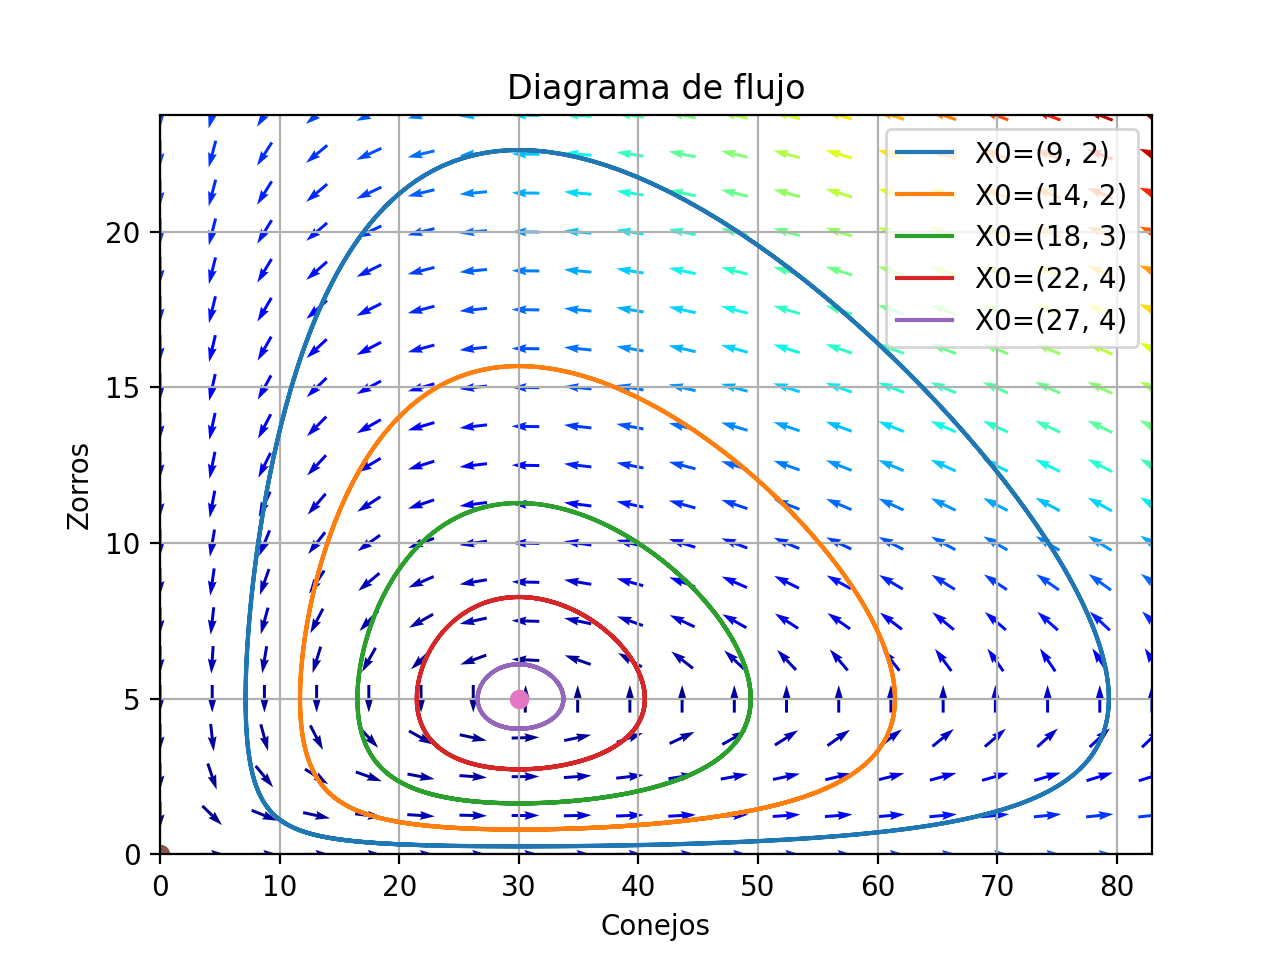
\includegraphics[width=\textwidth]{Figure_1.png}
\caption{Diagrama de flujo Zorros vs. Conejos}
\label{fig:Figure_1.png}
\end{figure}

En este gráfico podemos observar comportamientos del sistema para algunos valores iniciales . Las curvas nos dicen como evolucionan en el tiempo ambas especies. Por ejemplo, si tomamos la curva mas exterior (color azul), donde los valores iniciales son 27 conejos y 4 zorros,  podemos observar que los conejos llegan a su máximo (79) y comienzan a decrecer debido al aumento en el numero de zorros.
Hasta aquí, los zorros crecían de manera lenta con respecto a los conejos, debido a que no hay demasiados zorros para frenar el avance de los conejos. Sin embargo, cuando ya hay suficiente comida para los zorros, estos comienzan a crecen de manera mucho mas rápida para llegar a su máximo (30). Luego de aquí, ambas especies empiezan a decrecer. Esto es debido a que hay demasiados zorros y pocos conejos en el espacio. Una vez que la población de zorro entra en un declive, la población de conejos vuelve a recuperarse para repetir este ciclo a medida que avanza el tiempo.

Dado que en este sistema hay un predador y una preza, nos permite encontrar alguna configuración en que coexistan las especies por tiempo indefinido. 
Además, con esto podemos decir que cuando existe más de 5 zorros, la población de conejos comienzan a decrecer y la de zorros a aumentar. Cuando hay menos de 30 conejos, la población de zorro comienza a decrecer y a recuperarse la población de conejos. Y así sucesivamente. Esta relación se da para cualquier par de valores iniciales para las poblaciones que le demos a nuestro sistema (Sin cambiar las constantes del sistema)

\

Ahora nos interesa saber que cantidad de animales hay en un tiempo dado bajo ciertos valores iniciales. Si en el tiempo 0 contamos con 40 conejos y 9 zorros podemos resolver el sistema y encontrar una solución numérica para un tiempo dado.

\begin{figure}[H]
\centering
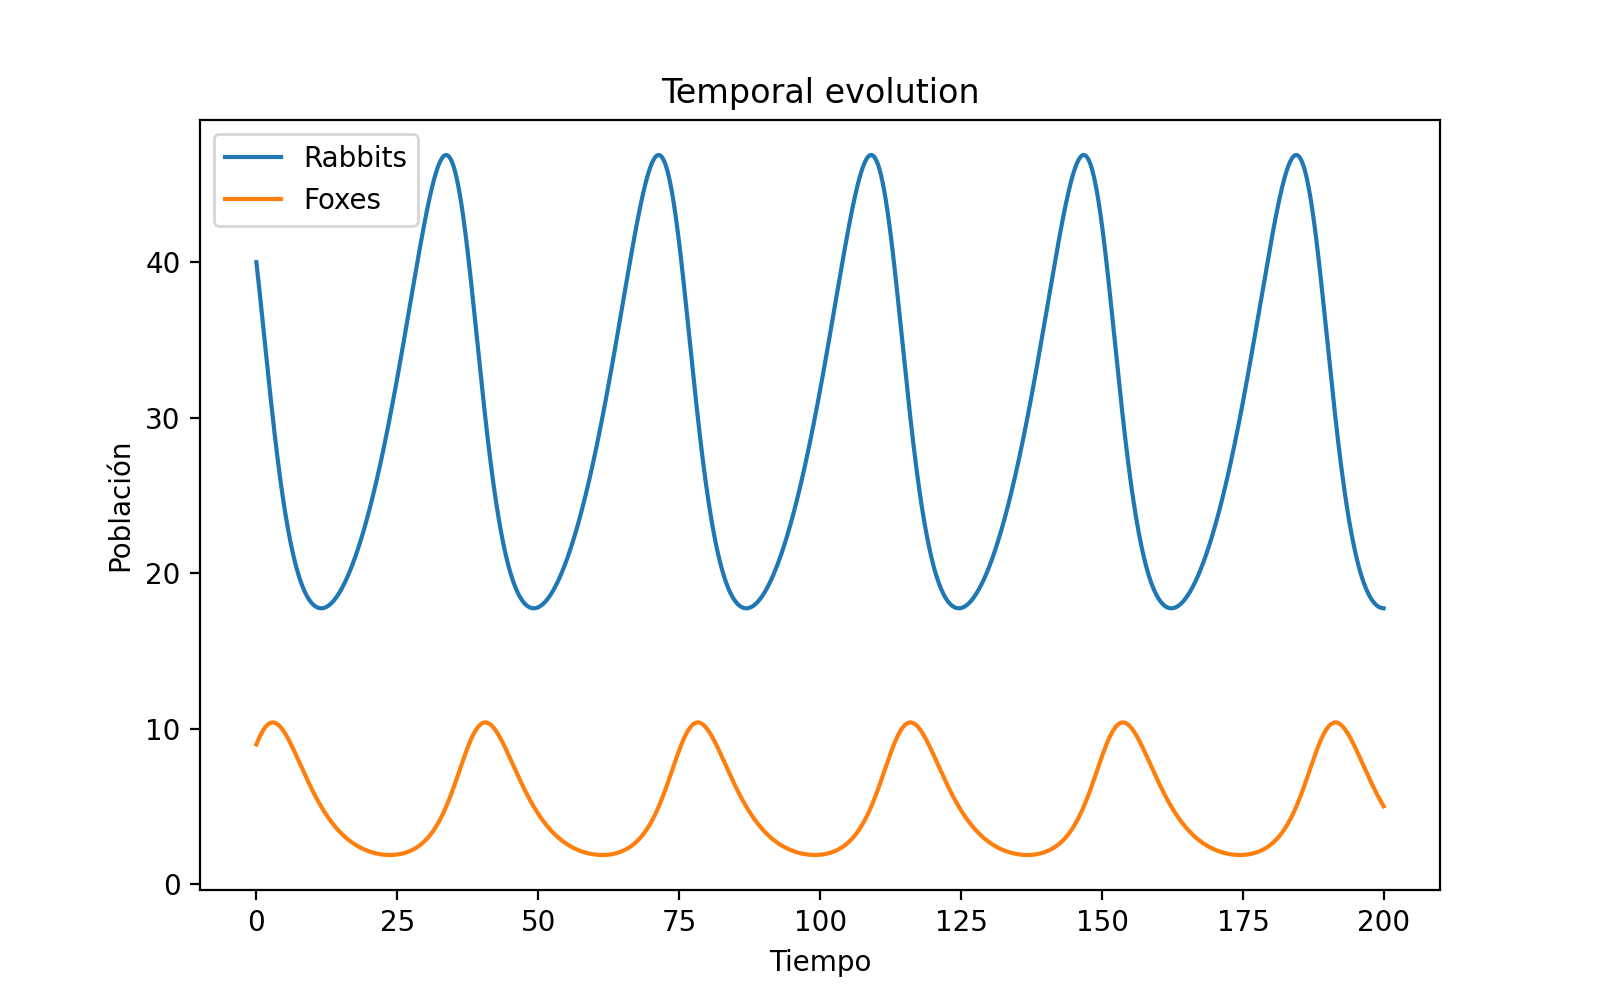
\includegraphics[width=\textwidth]{Figure_2.png}
\caption{Zorros vs. Conejos. Valores iniciales: C(0)=40 Z(0)=9}
\label{fig:Figure_2.png}
\end{figure}

El gráfico de arriba, nos muestra como es la relación cíclica que existe entre las poblaciones. Este se obtuvo tomando valores de tiempo de $0$ a $200$ e integrando con un paso de $0.05$.

Del mismo modo a lo explicado en el gráfico anterior, se observa que cuando la población de conejos llega al máximo, provoca un aumento en la población de zorros, lo que hace que la cantidad de conejos disminuya drásticamente. Luego, se produce una sequía en los alimentos para los zorros, haciendo que decaiga su numero de población. Esta caída en el numero de la población de zorros es mucho mas gradual que la de los conejos, donde se puede ver una caída en la cantidad de individuos más rápida. Una vez que la población de zorros empieza a caer, provoca que la población de conejo vuelva a crecer, repitiendo así el ciclo.
\


En el siguiente gráfico se puede observar el flujo del sistema para el problema de valor inicial descripto en el párrafo anterior.

\begin{figure}[H]
\centering
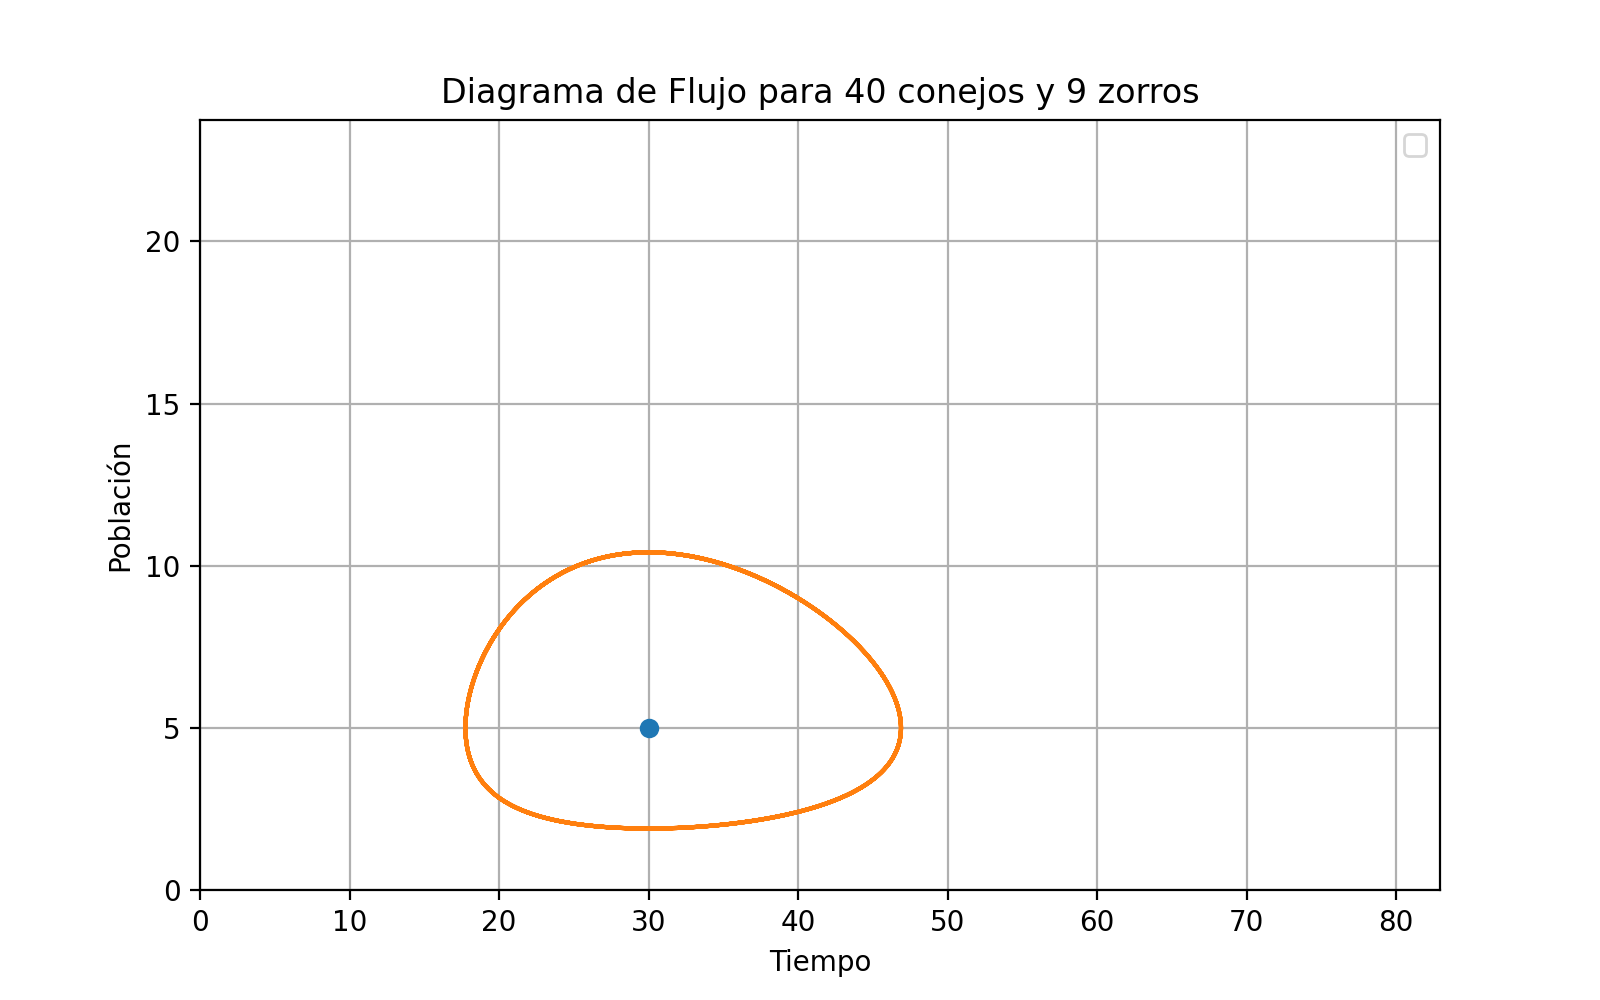
\includegraphics[width=\textwidth]{Figure_3.png}
\caption{Diagrama de flujo Conejos vs. Zorros.}
\label{fig:Figure_3.png}
\end{figure}

\


\textbf{Nota}: El práctico fue realizado en \textit{Python}, para integrar la ecuación diferencial ordinaria (ODE) se utilizo la función \textit{"solve\_ivp"} con el método "RK45" de la librería \textit{Scipy}.

    

\bibliographystyle{plain}
\bibliography{references}
\begin{itemize}
\item Nonlinear Dynamics and Chaos. Steven H Strogatz

\item https://steemit.com/steemstem/@masterwu/foxes-hunting-bunnies-population-modelling-with-the-predator-prey-equations

\item http://math.smith.edu/~callahan/cic/ch4.pdf

\item https://niko.roorda.nu/computer-programs/fox-rabbit-theoretical-model/
\end{itemize}

\end{document}
